\documentclass[11pt, oneside]{article}   	% use "amsart" instead of "article" for AMSLaTeX format
\usepackage{geometry}                		% See geometry.pdf to learn the layout options. There are lots.
\geometry{letterpaper}                   		% ... or a4paper or a5paper or ... 
%\geometry{landscape}                		% Activate for for rotated page geometry
%\usepackage[parfill]{parskip}    		% Activate to begin paragraphs with an empty line rather than an indent
\usepackage{graphicx}				% Use pdf, png, jpg, or eps� with pdflatex; use eps in DVI mode
								% TeX will automatically convert eps --> pdf in pdflatex		
\usepackage{amssymb}
\usepackage{amsmath}

\title{Spherical Cap - part I}
%\author{The Author}
\date{}							% Activate to display a given date or no date

\graphicspath{{/Users/telliott_admin/Dropbox/Tex/png/}}

\usepackage{listings,relsize} 
\lstloadlanguages{R} 
\lstset{language=R,basicstyle=\smaller[1],commentstyle=\rmfamily\smaller, 
  showstringspaces=false,% 
  xleftmargin=4ex,literate={<-}{{$\leftarrow$}}1 {~}{{$\sim$}}1} 
\lstset{escapeinside={(*}{*)}}   % for (*\ref{ }*) inside lstlistings (S code) 
\begin{document}

\maketitle
%\section{}
% \subsection*{R code}
% \begin{lstlisting}  \end{lstlisting}
% \begin{center} 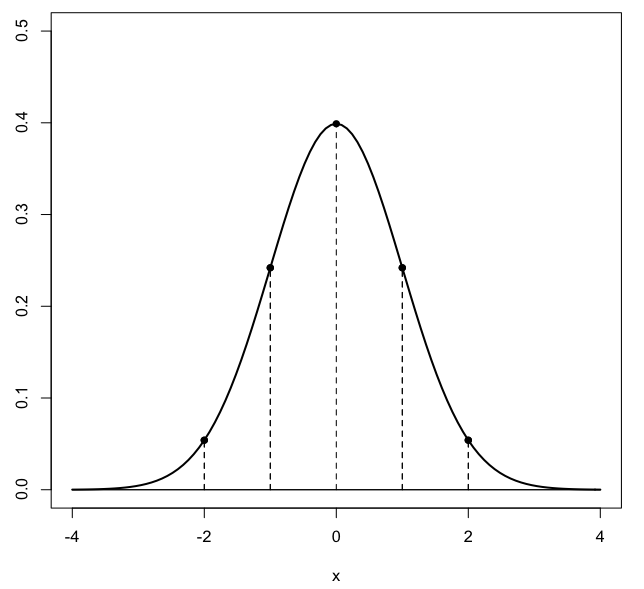
\includegraphics [scale=0.4] {gauss3.png} \end{center}
% \begin{bmatrix} a  &  b \\ c  &  d \end{bmatrix}
% \bigg |_

\large
\noindent
In this short write-up I want to derive the formula for the volume of a spherical cap.  This is the solid obtained by slicing off a part of a sphere with a plane. 
\begin{center} 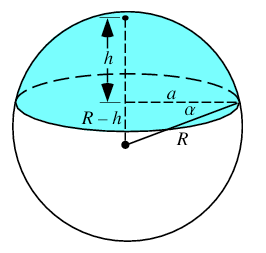
\includegraphics [scale=0.6] {spherical_cap.png} \end{center}
The formula we will derive is 
\begin{equation}
\boxed{V_{cap} = \frac{1}{3} \pi h^2(3R - h)}
\end{equation}
or equivalently
\[ V = \pi(Rh^2 - \frac{1}{3} h^3 )\]
We can see that this equation makes sense for the extreme case where $h=R$.  We get 

\[ V = \frac{1}{3} \pi R^2(3R - R) =   \frac{2}{3} \pi R^3 \]

\subsection*{Surface area of the sphere}
Let's begin by remembering the formula for the surface area of the sphere
\[ A = 4 \pi R^2 \]
Archimedes has a derivation of this in \emph{On the Sphere and Cylinder} which is explained in Dunham's book \emph{The Mathematical Universe}.  I'd prefer not to take that detour here, but note that calculus provides a simple proof, starting from the formula for the volume of a sphere
\[ V= \frac{4}{3} \pi R^3 \]
Suppose we take a sphere of radius $r$.  (I use $r$ here because for just this part, the radius will be a variable).  If we increase the radius by a little bit $dr$, then how does the volume change?  It changes exactly like the surface area!  That is
\[ dV = A \ dr \]
\[ A = \frac{d}{dr} \ V = \frac{d}{dr} \ \frac{4}{3} \pi r^3 = 4 \pi r^2 \]

Another way to see this is to break up the entire surface area of the sphere into small cones, each with area dA (almost flat) and height $R$.  The volume of one cone is
\[ \frac{1}{3}R \ dA \]
If we add up the volumes of all the little cones from the entire sphere we will have the volume of the sphere
\[ \frac{1}{3}R \ A \]
but we already know this is just $4/3 \pi R^3$,
so clearly
\[ \frac{1}{3} RA = \frac{4}{3}\pi R^3 \]
\[ A = 4 \pi R^2 \]

\subsection*{Volume of the sphere using calculus}

A modern way to do this is by integration of slices (from Strang)
\begin{center} 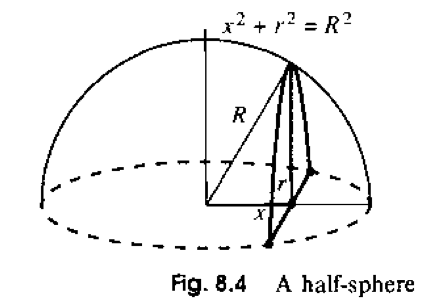
\includegraphics [scale=0.6] {sph_slices.png} \end{center}
At each value of $x$, the cross-section of the hemisphere (radius $R$) is a half-circle with radius $r$ such that
\[ x^2 + r^2 = R^2 \]
the area of this hemisphere cross-section is
\[ A = \frac{1}{2} \pi r^2= \frac{1}{2} \pi (R^2 - x^2) \]
For the whole sphere, each cross-section is a circle with area
\[ A =  \pi r^2= \pi (R^2 - x^2) \]
For the volume, we just add up all these slices.  To make it simple, take $x$ from $x=-R \to x=R$ 
\[ V =  \int_{-R}^{R} \pi (R^2 - x^2) \ dx \]
\[ V =  \pi \int_{-R}^{R}  (R^2 - x^2) \ dx \]
\[ =  \pi \ [ \ R^2x - \frac{1}{3}x^3 \ ] \ \bigg |_{-R}^R \]
\[ =  \pi \ ( R^3 - \frac{1}{3}R^3 -(-R)^3 + \frac{1}{3}(-R)^3  \]
\[ =  \frac{4}{3}\pi R^3 \]

\subsection*{Volume of the spherical cap}

For the cap, just change the lower limit of integration to $x=R-h$  !!  
\begin{center} 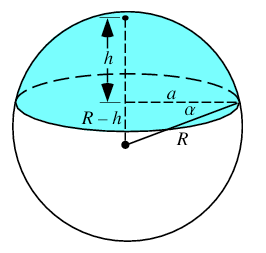
\includegraphics [scale=0.6] {spherical_cap.png} \end{center}
We need to evaluate
\[ V = \pi \ [ \ R^2x - \frac{1}{3}x^3 \ ] \ \bigg |_{R-h}^R \]
Leave aside the factor of $\pi$, and break the expression into two parts 
\[ R^2x  \ \bigg |_{R-h}^R - \frac{1}{3} x^3  \ \bigg |_{R-h}^R \]
For the left term we get
\[ R^3 - R^3 + R^2h = R^2h\]
For the right side we get
\[ -\frac{1}{3} R^3 + \frac{1}{3}(R-h)^3 ) \]
\[=  -\frac{1}{3} R^3 + \frac{1}{3} R^3 - R^2h + Rh^2 -\frac{1}{3} h^3 \]
Adding left and right terms together, the $R^2h$ cancel, and we have finally
\[ V = \pi (Rh^2 - \frac{1}{3} h^3) \]
Factoring out $\frac{1}{3} h^2$
\[ V = \frac{1}{3} \pi h^2 (3R -h) \]
which is the formula we gave at the top.

\subsection*{Volume of a spherical belt}
We can calculate the volume of any spherical belt by using the appropriate limits of integration.  For example, the belt from $r=0 \rightarrow r = R-h$ has volume
\[ V = \pi \ [ \ R^2x - \frac{1}{3}x^3 \ ] \ \bigg |_{0}^{R-h} \]
Leaving the $\pi$ aside for now
\[ R^2(R-h) - \frac{1}{3}(R-h)^3 \]
\[ R^3 - R^2h - \frac{1}{3}(R^3 - 3R^2h + 3Rh^2 - h^3) \]
\[ \frac{2}{3}R^3 - Rh^2 + \frac{1}{3} h^3  \]
With the factor of $\pi$
\[ V = \pi ( \frac{2}{3}R^3 - Rh^2 + \frac{1}{3} h^3 )  \]
Adding the cap and the belt together:
\[ V_{tot} =  \pi( Rh^2 - \frac{1}{3}h^3 + \frac{2}{3}R^3 - Rh^2 + \frac{1}{3} h^3) \]
Almost everything cancels
\[ V_{tot} =  \pi( \frac{2}{3}R^3) \]
The cap and the belt together make up a hemisphere.




\end{document}  